% !TEX TS-program = lualatex
%\documentclass[handout]{beamer}
\documentclass{beamer}
\input{../common/misomva}
\newcommand{\misoclasstinytitleslide}{Partially based on material by:  Ulrike von Luxburg, \\[-1em] Gary Miller, Doyle \& Schnell, Daniel Spielman}
\newcommand{\misoclassdate}{}
\usetikzlibrary{graphs}

\begin{document}
% Topic-specific title slide

\newcommand{\topictitle}{Spectral Clustering: Background}

\newcommand{\topicsubtitle}{Motivation and Problem Setting}

\MakeTopicSlide

%%%%%%%%%%%%%%%%%%%%%%%%%%%%%%%%%%%%%%%%%%%%%%%%%%%%%%%%%%%%
\begin{frame}
\frametitle{How to rule the world: ``AI'' is here}
\centering

\includegraphics[width=0.3\columnwidth]{obama1}\moveb
{\tiny
\url{https://www.washingtonpost.com/opinions/obama-the-big-data-president/2013/06/14/1d71fe2e-d391-11e2-b05f-3ea3f0e7bb5a_story.html} \moves
\url{https://www.technologyreview.com/s/509026/how-obamas-team-used-big-data-to-rally-voters/}\\
Talk of Rayid Ghaniy: \url{https://www.youtube.com/watch?v=gDM1GuszM_U}
}
\end{frame}
%%%%%%%%%%%%%%%%%%%%%%%%%%%%%%%%%%%%%%%%%%%%%%%%%%%%%%%%%%%%

%%%%%%%%%%%%%%%%%%%%%%%%%%%%%%%%%%%%%%%%%%%%%%%%%%%%%%%%%%%%
\begin{frame}
\frametitle{Application of Graphs for ML: Clustering}
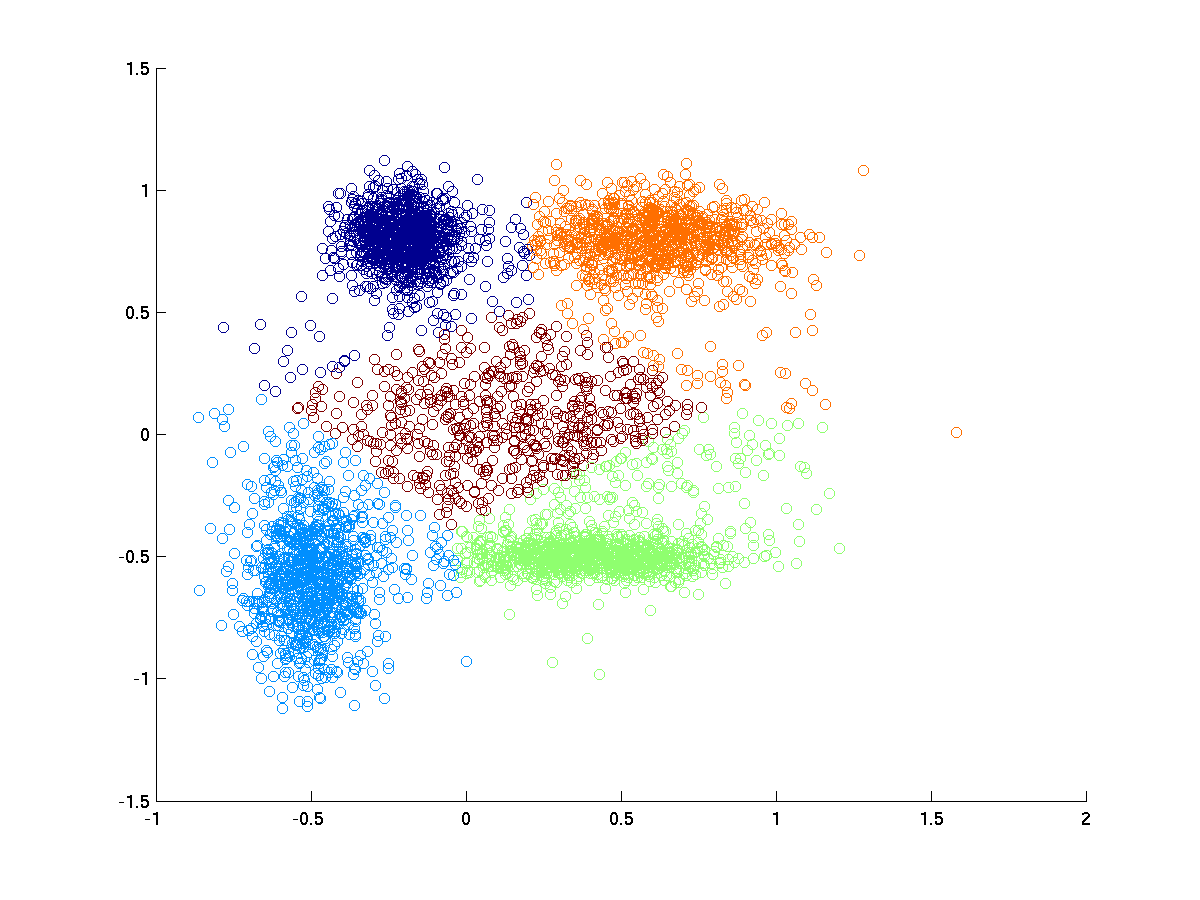
\includegraphics[width=0.45\columnwidth]{../img/compactness}
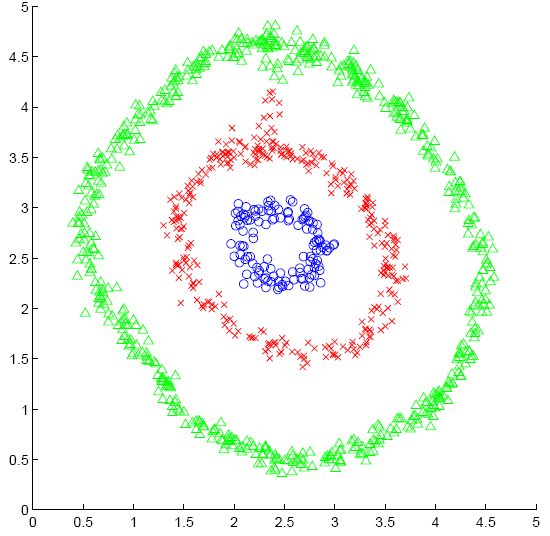
\includegraphics[width=0.45\columnwidth]{../img/connectivity}
\end{frame}
%%%%%%%%%%%%%%%%%%%%%%%%%%%%%%%%%%%%%%%%%%%%%%%%%%%%%%%%%%%%

%%%%%%%%%%%%%%%%%%%%%%%%%%%%%%%%%%%%%%%%%%%%%%%%%%%%%%%%%%%%
\begin{frame}
\frametitle{Background: Clustering}

\begin{itemize}[<+-| alert@+>]\addtolength{\itemsep}{0.75\baselineskip}
\item \questionbox{What do we know about the \gcol{clustering} in general?}
\begin{itemize}
\item ill defined problem (different tasks $\to$ different paradigms)
\item ``I know it when I see it''
\item inconsistent (wrt.~\href{https://www.cs.cornell.edu/home/kleinber/nips15.pdf}{\underline{Kleinberg's axioms}})
\begin{itemize}[<handout:0>]
\item \grcol{scale-invariance, richness, consistency}
\end{itemize}
\item number of clusters $k$ need often be known
\item difficult to evaluate
\end{itemize}
\item \questionbox{What do we know about \gcol{$k$-means}?}
\begin{itemize}
\item ``hard'' version of EM clustering
\item sensitive to initialization
\item optimizes for \gcol{compactness}
\item yet: algorithm-to-go
\end{itemize}
\end{itemize}


\end{frame}
%%%%%%%%%%%%%%%%%%%%%%%%%%%%%%%%%%%%%%%%%%%%%%%%%%%%%%%%%%%%

\MakeLastSlide
\end{document}
